\chapter{ACTUAL WORK} % Main chapter title
\label{ChapterActualWork} % For referencing the chapter elsewhere,
% use \ref{Chapter1}

\section{Methodology for the Study}\index{Methodology}
By implementing the RiskWise system based on a multi-stage process,
an unstructured legal document like a Terms of Service is converted
to a structured knowledge representation, which is accompanied by
user-related risk insights. 

Unlike in the research methodology as described in Chapter 2, which is more focused on explaining issues related
to the conceptual design and research strategy, in this section, a description of the operational workflow
developed in the course of creating the framework is presented.
The operational workflow is designed to process raw legal texts and generate understandable output in a
systematic manner through a set of analytical steps.

The process begins with a "document ingestion part" in which the user can upload documents containing "Terms of Service" in a web-based way.
The proposed service aims to assess the documents uploaded by the user, as well as documents in multiple formats.
The text extraction part of the documents will be performed, keeping the logical order of the documents.

Then, a semantic segmentation component is applied to text data in which a coherent chunking of text is
performed at clause-level granularity.
The mechanism for text segmentation is designed to maintain context and facilitate text retrieval and
reasoning, which is a subsequent step.
Subsequently, a semantic embeddings component is applied in which embeddings for each segmented text
component are generated using embedding models designed for legal text and its subtle semantics. 

These embeddings are vectors of textual
meaning allowing similarity-oriented retrieval over semantically
related clauses even beyond lexical overlap. The generated embeddings
are stored in a vector indexing\index{Vector Database} mechanism that allows fast and
scalable nearest-neighbor search during analysis and query processing.

These embeddings are vectors of textual
meaning allowing similarity-oriented retrieval over semantically
related clauses even beyond lexical overlap. The generated embeddings
are stored in a vector indexing\index{Vector Database} mechanism that allows fast and
scalable nearest-neighbor search during analysis and query processing.

Apart from using the model for the embedding of the generation, the language model can also be used for extracting subject-predicate-object triples\index{Triple Extraction} from the text segments, which can form a basis for representing the knowledge graph\index{Knowledge Graph}. The representation of the knowledge graph can give an account of the relational dependency of the entities such as users, service providers, permissions, obligations,
contractual actions.By connecting the
components of the documents, the knowledge graph enables the
relational analysis that can connect the context beyond the apparent
textual similarity.

In addition with the aim of using the semantic knowledge as well as the 
knowledge of the structure, a new hybrid retrieval technique\index{Hybrid Retrieval} 
has been developed that can include vector similarity 
search\index{Vector Similarity Search} as well as graph 
traversal\index{Graph Traversal}. This will enable one to 
retrieve not only contextually relevant information but also 
relationally related information in a way that enriches the context of 
the information for a comprehensive analysis thereof. The hybrid-technique 
in information retrieval, as proposed above, will enable one to 
transcend the limitations of different information retrieval 
techniques and enrich the context of the information.

Lastly, the contextual information retrieved is processed by a
generative reasoning module\index{Generative Reasoning} set up for risk-based processing\index{Risk Analysis}. This
module provides analyses of the context, and uses it to categorize
potential risky clauses\index{Clause Detection}, to make severity judgments to help derive a
score and categorize risk-types and to provide explainable summaries\index{Explainable AI}
in natural language based on evidence retrieved. Combining retrieval
grounding with generative reasoning, the system's outputs are
interpretable, contextually aware, and consistent with document details.

The RiskWise system manages the efficient, explorable and
context-sensitive analysis of contractual documents through the
multi-step and coordinated approach, making it possible to process
intricate legal agreements into general users’ accessible results.

\section{Experimental  Work}
The experimental stage of the project was characterized by iterative
evaluation of different methods for automated clause detection and
risk identification. The initial experimentation stages involved experimenting with the transformer models for ques-tion answering for clause extraction. This provided the initial insights for what these models can
achieve for legal text understanding. Other experimentation stages involved validating different
components of different models, including the accuracy of the semantic chunking schemes, embedding-based retrieval methods, and knowledge graphs.

ToS documents from a variety of digital platforms were examined and processed in the pipeline to analyze
system robustness for different document structures and legal formulations using multiple ToS documents as
case studies.
Overall, the comparative analysis of the retrieval results confirms that hybrid retrieval mechanisms achieved
greater contextual completeness than purely semantic retrieval.

In addition, testing the local and cloud-based inference modes facilitated a comparison in terms of performance trade-offs in terms of computational efficiency and response latency.
Experiments were conducted to facilitate fine-tuning and validation of the proposed hybrid GraphRAG framework.

\section{Analytical Work}
We manually reviewed the retrieved clauses for semantic similarity search for contextually appropriate
segments corresponding to user queries and analysis tasks.
The extracted relationships were checked to be accurate in terms of logical consistency to ensure that the
extracted relationships corresponded to that of identified entities.

The results obtained from graph traversal\index{Graph Traversal} were validated to ensure that the contexts provided in the relational contexts gave additional information apart from the results provided in the vector retrieval results.
The results obtained from the risk analysis\index{Risk Analysis} module were validated in terms of their understandability, accuracy and consistency with the document content.

The severity scores and the risk categories were also validated to ensure that they addressed the issues related to the interests, such as changes in contracts, liabilities and permissions related to data usage. Thus, the context grounding has been appropriately achieved for the interpretation of the user.

\section{Modeling, Analysis \& Design}
A modular and multi-tiered architecture is used to represent the
system.
This system has its end-user interface layer, where there is the web interface and the presentation layer, the system that processes the provided information, the processing layer, and the storage system itself, the storage layer.
The presentation layer has the role of designing a user interface that is not just intuitive but also friendly.
The processing layer is where the intelligence of the system can be found.
This system has six different modules in the processing layer of the system and these are the text extraction module, the semantic chunking module, the embeddings module, the knowledge graph module, the hybrid retrieval module and the generative reasoning module.
All the modules in the system are independent of each other, though the objective of all the modules in the system is the same, at least in the procesing layer of the system.
This storage layer has the graph database\index{Graph Database} itself.

Furthermore, this design aids in retrieval and reasoning by attaching
semantic and structural information together. 
The key factors in how
the system was designed are modularity, scalability and clarity.
Because the system separates the vector and graph representation of
information, different retrieval options can be utilised. 

The modular
processing components can accommodate future growth and enhancements
to the processing models without the need to redesign the entire system.

\begin{figure}[h]
  \begin{center}
    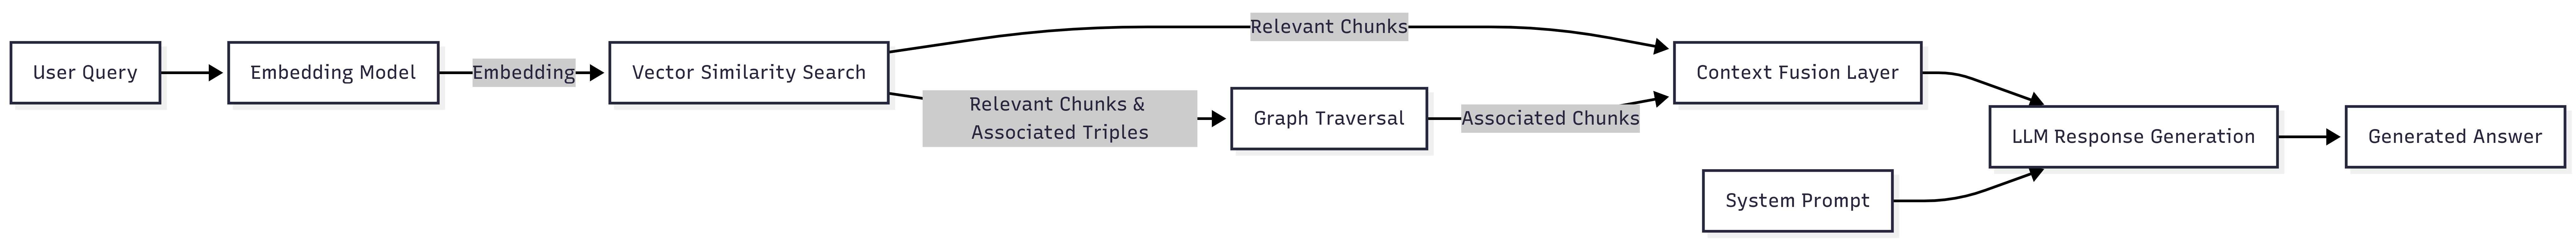
\includegraphics[width=0.8\textwidth]{Figures/forward_pass_through_architecture.png}
    \caption{Retrieval Mechanism}
    \label{fig:a}
  \end{center}
\end{figure}

\begin{figure}[h]
  \begin{center}
    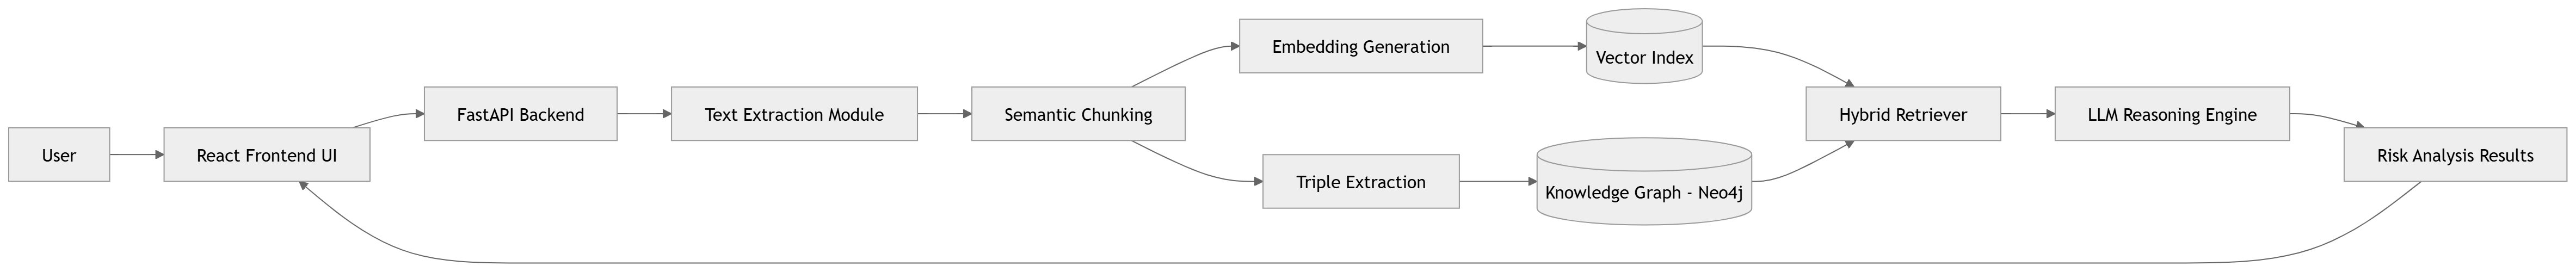
\includegraphics[width=0.8\textwidth]{Figures/frontend.png}
    \caption{Frontend Architecture}
    \label{fig:b}
  \end{center}
\end{figure}

\section{Prototype \& Testing}
To demonstrate end-to-end analysis functionality, the RiskWise system
has been created as a prototype consisting of a web user interface
integrated with back-end capabilities to process and analyze
documents. Users can upload ToS documents, check their processing
status, view risk results classified by type, and interact with the
system using a conversational query interface. The prototype testing
was performed by simulating various user scenarios (e.g. uploading a
  document, displaying risk analysis results, and answering queries in
context). Functional testing was performed to verify that each stage
of the pipeline was executed correctly and integration testing was
conducted to verify that the front-end and back-end systems
interacted correctly. For performance testing, processing time was
measured for different document sizes and inference configurations to
ensure there were expected differences in latency between local and
cloud executions. Unsupported formats and invalid inputs were
included in the testing to validate error handling and confirm
strength of the system. The overall prototype testing indicated
compliance with the functional correctness and usability requirements
of the system.

\section{Algorithms and Flowcharts}
The operational workflow of the RiskWise system can be represented
through algorithmic steps describing the document analysis pipeline.

\textbf{Algorithm: RiskWise Document Analysis Pipeline}
\begin{enumerate}
  \item Start
  \item Accept document upload from user
  \item Validate file format and generate document identifier
  \item Extract textual content from document
  \item Perform semantic segmentation into text chunks
  \item Generate embeddings for each chunk
  \item Store embeddings within vector index
  \item Extract knowledge triples from chunks
  \item Construct knowledge graph representation
  \item Perform hybrid retrieval combining vector similarity and graph traversal
  \item Provide retrieved context to generative reasoning module
  \item Identify risky clauses and assign severity scores
  \item Generate explainable summaries and present results
  \item Enable interactive user querying
  \item End
\end{enumerate}

\begin{figure}[H]
  \begin{center}
    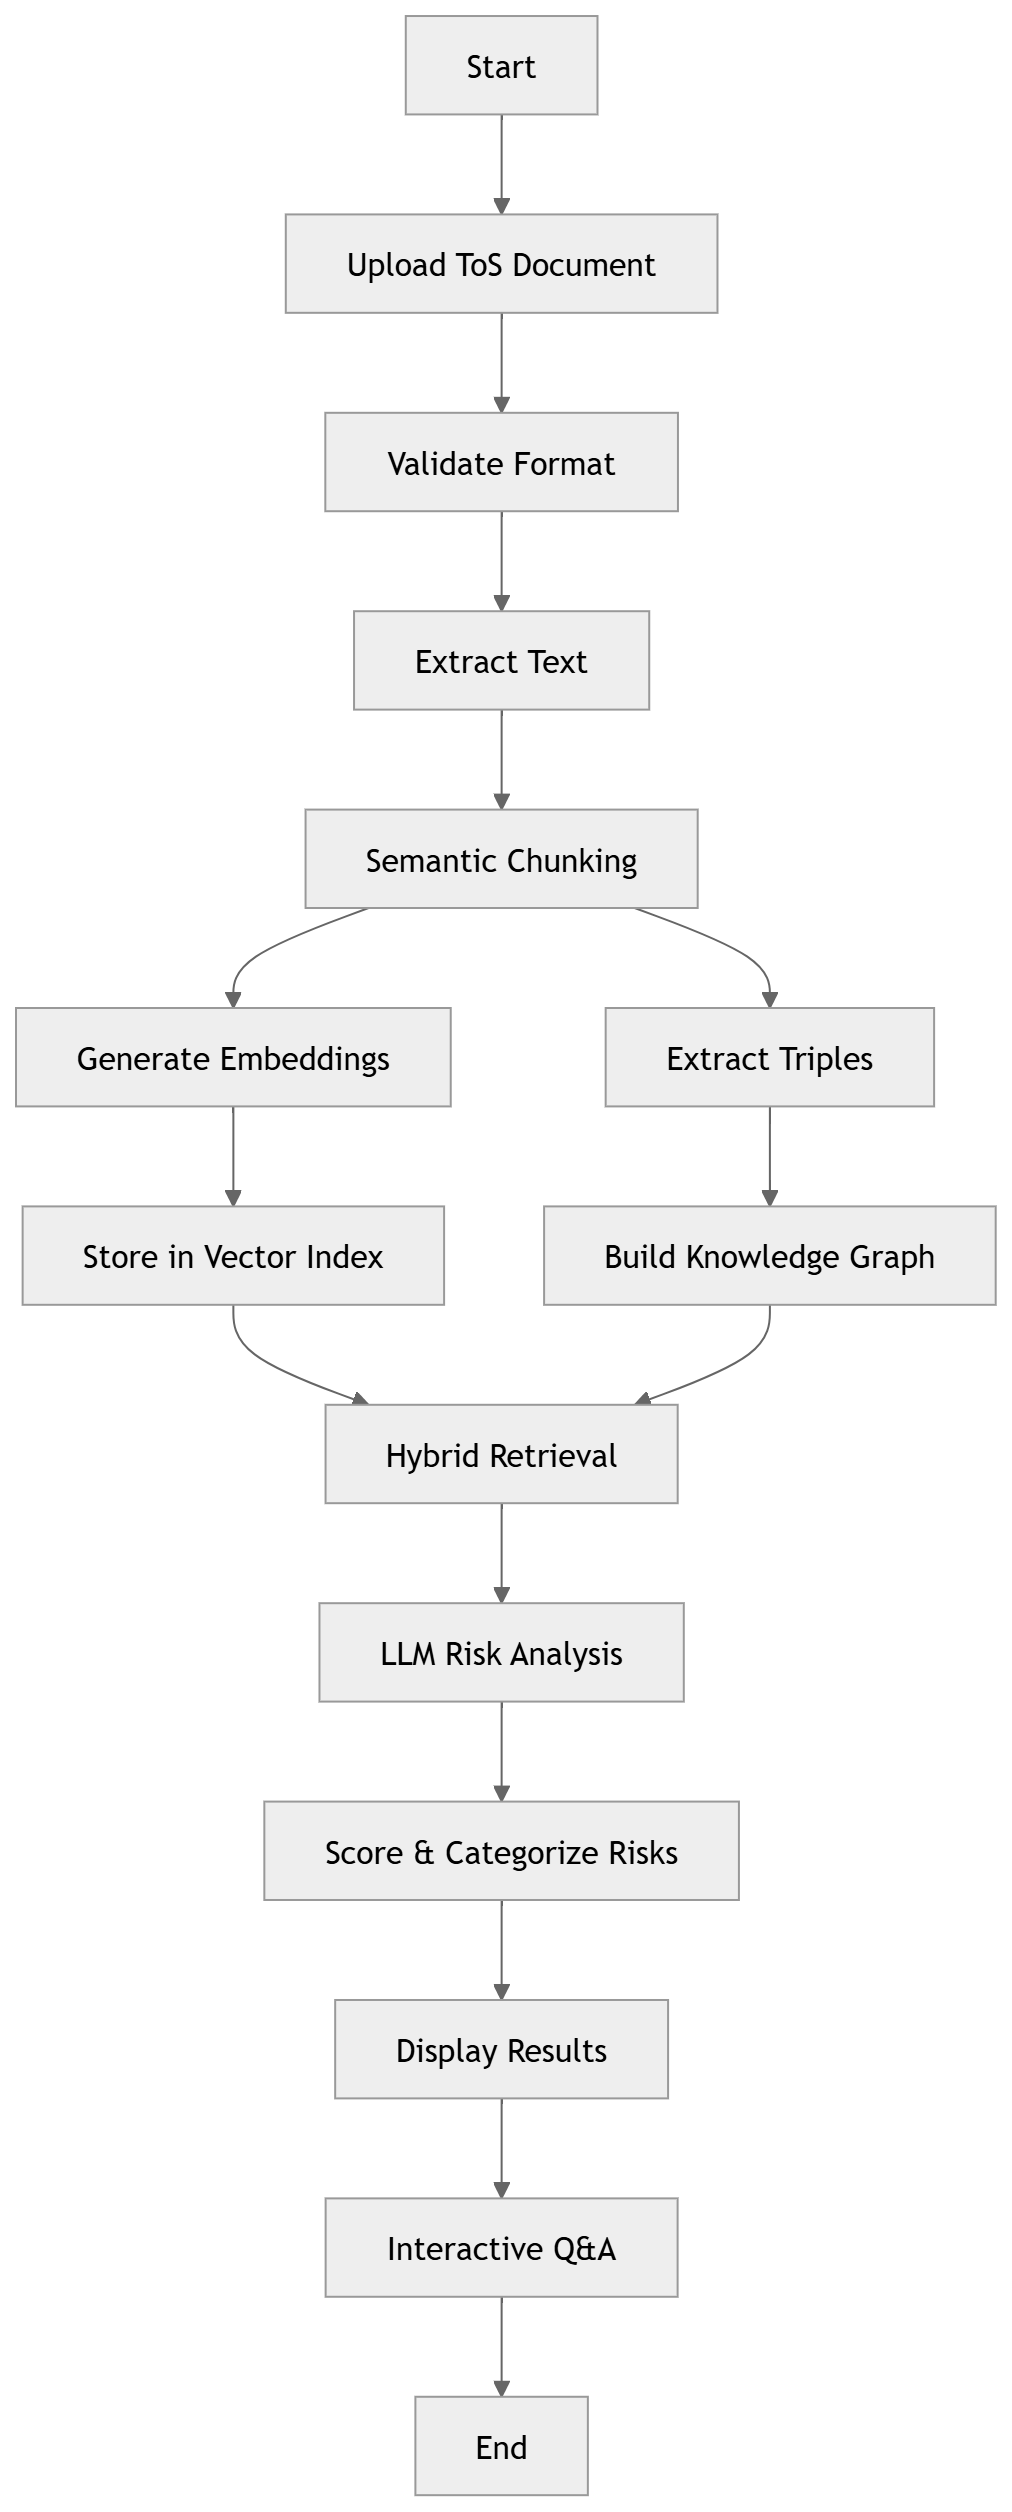
\includegraphics[scale=0.1]{Figures/doc_proc.png}
    \caption{Document Analysis}
    \label{fig:c}
  \end{center}
\end{figure}

\begin{figure}[H]
  \begin{center}
    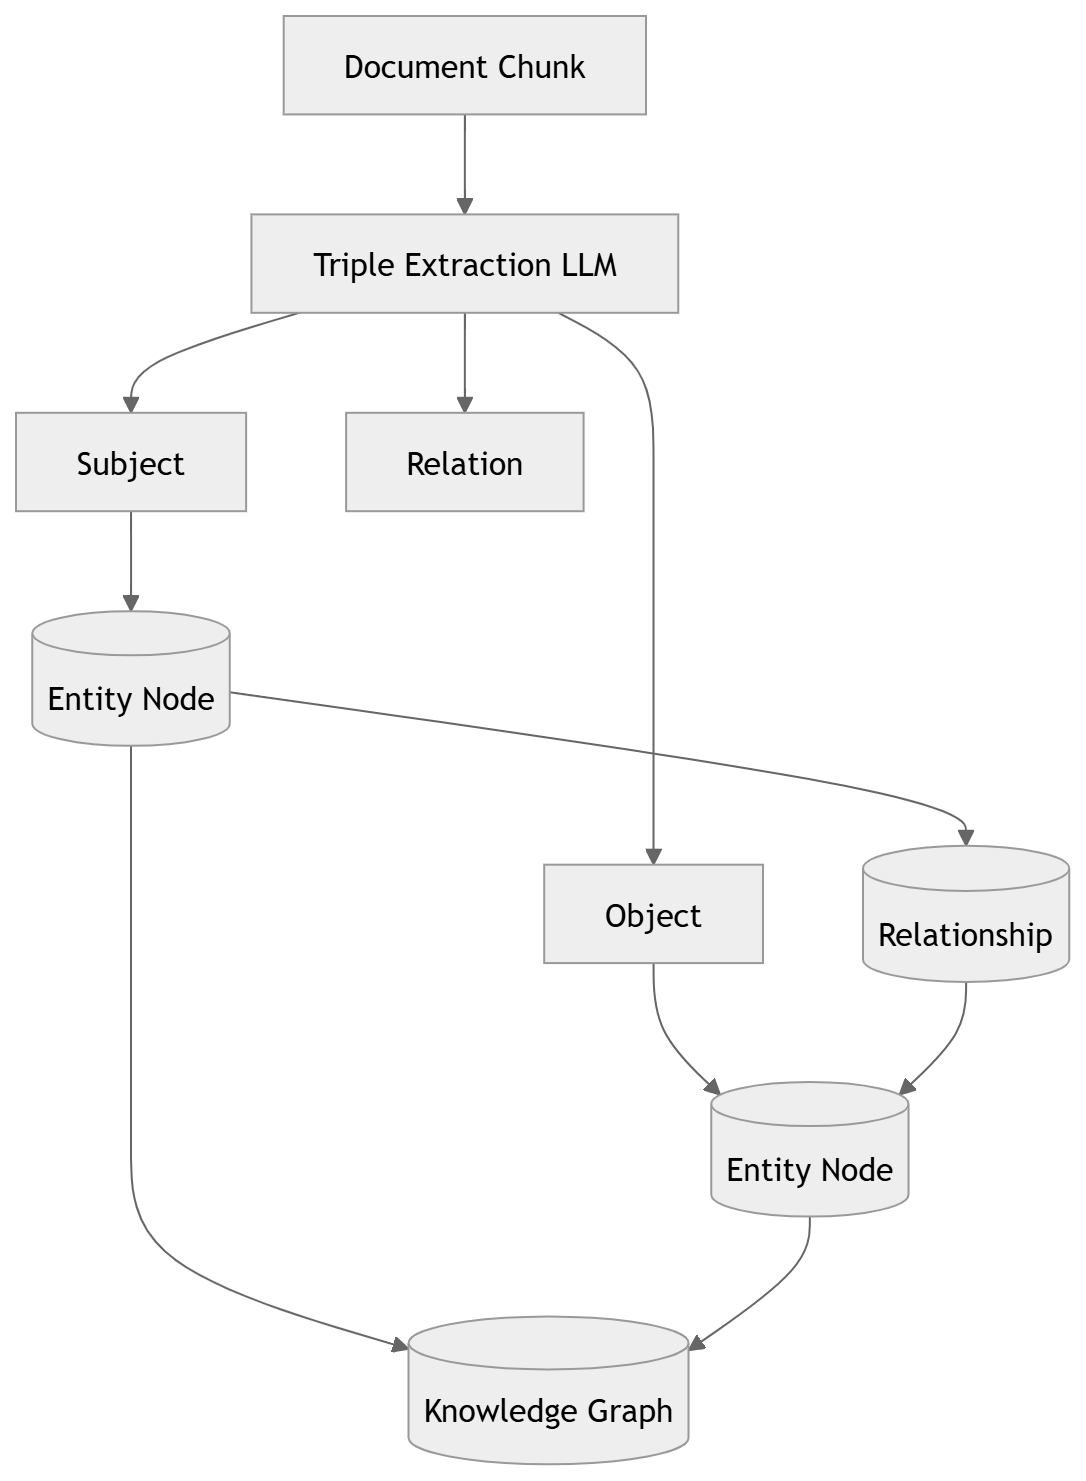
\includegraphics[scale=0.1]{Figures/triple_gen.png}
    \caption{Knowledge Graph Generation}
    \label{fig:d}
  \end{center}
\end{figure}

\section{Codes / Standards}
RiskWise system was developed in accordance with recognized standards
of software engineering, with established tools in data handling,
industry-oriented practices and standard methods to maintain
reliability, integrity, maintainability, compatibility and
responsible behavior. Due to being a work in the automated legal
report inspection area, transparency and modularity and
explainability at all stages of development were the focus of the code.
\\

\textbf{Standards for Software Development}

The framework was mostly developed in Python code and was written in
a standard coding fashion to make it easier to read, collaborate, and
maintain. To make sure that the code was readable, standard naming
and modular programming practices, as well as organizing modules in
an organized way, were followed. The main functional modules, such as
document processing, embedding generation, knowledge graph
construction, retrieval logic, and reasoning modules, were developed
as separate modules.
\\

\textbf{API and Integration Standards}

Both front-end-side and backend layer functionality of the
interaction between pieces of system programming was handled by
creating code on, for example, RESTful API principles of the RESTful
API framework to enable communication between API components. Data
exchange was done through standard HTTP request-response mechanisms,
and JSON format which the data was used as the main data format
because of its lightweight layout and the ability to use this media
type for its lightweight and applicable platform. These integration
methods were leveraged to facilitate easy integration of
document-based service-ingestion systems, retrieval pipelines,
retrieval methods, and interfaces in the user interface components
were optimized by seamless orchestration.
\\

\textbf{Data Management and Data Protection Standards}

Since user uploaded documents could include potentially proprietary
contractual information, privacy-aware data handling practices were
accounted for in the system development. We used uploaded documents
as workstopped files and did not keep superfluous metadata and used
temporary caching mechanisms for each iteration of the same document
to enhance performance. The approach is focused on minimizing data
and treating analysis artifacts with control; both data protection
principles and ethical AI development principles are well-accepted.
\\

\textbf{Ethics in AI and Responsible Usage Guidelines}

The RiskWise system was developed with a focus on responsible AI use.
The returns on risk analysis are structured in a way that is based on
the document context retrieved to mitigate the issue of hallucination
in terms of how the generated explanations can be made more
transparent in terms of interpretation. The system has a purposeful 
approach to its usage in the promotion of user awareness rather than 
legal advice and the results produced in the form of informative insights.
\\

\textbf{NLP Standards and Knowledge Representation Standards}

Normalization methods in NLP, such as text normalization, sentence
segmentation, and semantic chunking, are performed on a periodic
basis for data preparation in NLP. The embedding methods used were
based on the transformer modeling paradim that has been popular in
modern semantic retrieval models. Additionally, the development of
the knowledge graph was based on the subject predicate object
representation paradigm that has been widely used in knowledge
engineering, enabling data structure relationships in all document materials.
\\

\textbf{System Design and Documentation Standards}

Project documentation is guided by academic and engineering
documentation conventions for a modular system description,
architectural diagrams, algorithmic representation, experimental
verification and validation. We included flowcharts and system
diagram of system functionality, which will facilitate reproducible
and technically transparent design, so that the system design can be
understood, reviewed and extended by any future researcher or developer.
Following these coding, integration and operational conventions,
RiskWise system ensures enhanced reliability, scalability and
interpretability while ensuring the responsible procesing of user
provided contractual data. These behaviour all facilitate the
development of a scalable and resilient platform for in the automatic
interpretation of legal documents.

%\section*{Sample LaTeX Typesetting}

%\paragraph*{Figure} Vector Graphics EPS Format [Figure \ref{fig:fcmc1}]
%\begin{figure}[H]
%  \begin{center}
%    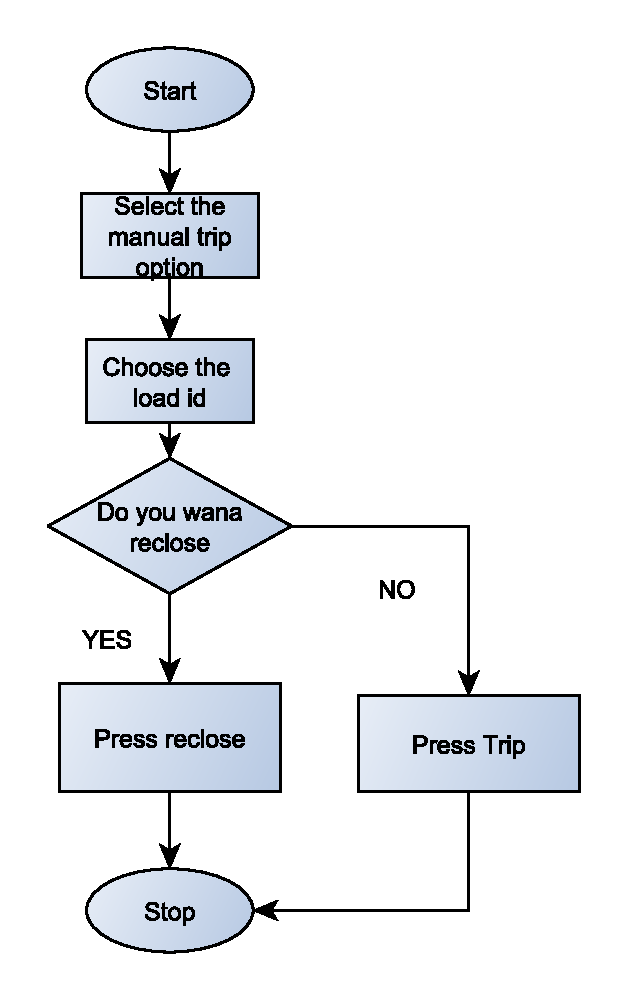
\includegraphics[scale=0.7]{Figures/manualtrip.eps}
%    \caption{Flowchart of Manual Controller}
%    \label{fig:fcmc1}
%  \end{center}
%\end{figure}
%
%This is shown in Figure \ref{fig:fcmc1}
%
%\paragraph*{Table} Refer [Table \ref{tab:sm}]
%\begin{table}[h]
%  \centering
%  \caption{Student Marks}
%  \begin{tabular}{rr}
%    \toprule
%    Name  & Marks \\
%    \midrule
%    Ajay  & 10 \\
%    Vinay & 20 \\
%    \bottomrule
%  \end{tabular}%
%  \label{tab:sm}%
%\end{table}%
%
%\paragraph*{Cross References: Citation, Index, Reference, Equation reference}
%This is the methodology for the entire project work which includes
%even the process of deciding on the project title, objectives
%\index{Ojectives}, etc. This is mandatory for MTech and optional for
%BTech)\cite{abcdef}. The data is shown in Table \ref{tab:sm}. The
%equation shown in Equation \eqref{Eq:eq123}
%
%\paragraph*{Inline Equation}
%This is my equation.
%$  f = ma \pm \alpha \Delta \left[ {
%  \begin{array}{*{20}{c}}
%    1 & \chi   \\
%    { - 1} & 0  \\
%\end{array}} \right] $
%,which is appearing in between some text.
%
%\paragraph*{Equation without Numbering}
%\begin{equation*}
%x = \frac{{ - b \pm \sqrt {{b^2} - 4ac} }}{{2a}}\
%\end{equation*}
%
%\paragraph*{Equation with Numbering}
%\begin{equation} \label{Eq:eq123}
%\dot X = \left[ {
%    \begin{array}{*{20}{c}}
%      1 & p  \\
%      2 & \alpha   \\
%\end{array}} \right]\left[ {
%    \begin{array}{*{20}{c}}
%      {{x_1}}  \\
%      {{x_2}}  \\
%\end{array}} \right] + Bu\
%\end{equation}
%
%\paragraph*{Algorithm Format}
%\begin{algorithm}
%\caption{Addition of two 8 bit numbers}\label{alg:add8bit}
%\begin{algorithmic}[1]
%  \\ Start
%  \\ Input a and b
%  \\ c=a+b
%  \\ Output c
%  \\ stop
%\end{algorithmic}
%\end{algorithm}
%
%\paragraph*{Enumeration Format}
%The following are the different flavor of Tex systems
%\begin{enumerate}
%\item TeXLive TeX System
%  \begin{enumerate}
%    \item TeXLive for Windows
%      \begin{enumerate}
%        \item TeXLive
%        \item ProTex
%      \end{enumerate}
%    \item MacTeX for Mac
%  \end{enumerate}
%\item MikTeX TeX System
%\end{enumerate}
%
%\paragraph*{Bullets Format}
%The following are the advantages of LaTeX,
%\begin{itemize}
%\item {\LaTeX} is highly portable and free.
%  \begin{itemize}
%    \item Contribute to TUG
%    \item Promote Free Softwares
%  \end{itemize}
%\item Operating-system independent.
%\item Complex scientific documents can be created
%  automatically.
%\item High quality math typesetting.
%\end{itemize}

%\paragraph*{Program Inclusion} Program file present in other
%directory can be embedded into the report.
%\lstinputlisting{Files/code.asm}
%
%\paragraph*{Verbatim Text} Include text as it is.
%\\
%The additional database schema is shown below which is used to store
%all the configuration and transaction data.
%\begin{verbatim}
%CREATE TABLE `controller_config` (
%`load_id` int(11) NOT NULL,
%`ct_constant` double DEFAULT NULL,
%`pt_constant` double DEFAULT NULL,
%`samples` int(11) DEFAULT NULL,
%`delay` double DEFAULT NULL,
%PRIMARY KEY (`load_id`)
%) ENGINE=InnoDB DEFAULT CHARSET=utf8;
%SELECT * FROM loadcontroller.load_details;
%\end{verbatim}
